\section{Motivation}\label{sec:motivation}

As being said in the \autoref{ch:introduction}, we try to describe more possible shapes with adding a third \gls{pdf}.
To illustrate that, we plotted some of the shapes which are now possible but were not possible before.
To be able to draw those plots, we are just using two variables, $w$, the upward wind, and $\theta_l$, the liquid water potential temperature.
First, we fix the following variables: $w_1 = 5$, $w_2 = -5$, $\theta_{l1} = 5$, $\theta_{l2} = -5$, $\alpha = 0.5$.
To illustrate how the binormal model handles strong winds, let us consider a scenario with strong upward winds at two locations $w_1$, as well as at $w_2$.
The way the current binormal model would model this could look like \autoref{fig:plot1}, where $\sigma_w = 2$, $\sigma_{\theta_l1} = 2$, $\sigma_{\theta_l1} = 2$.

\begin{figure}
    \centering
    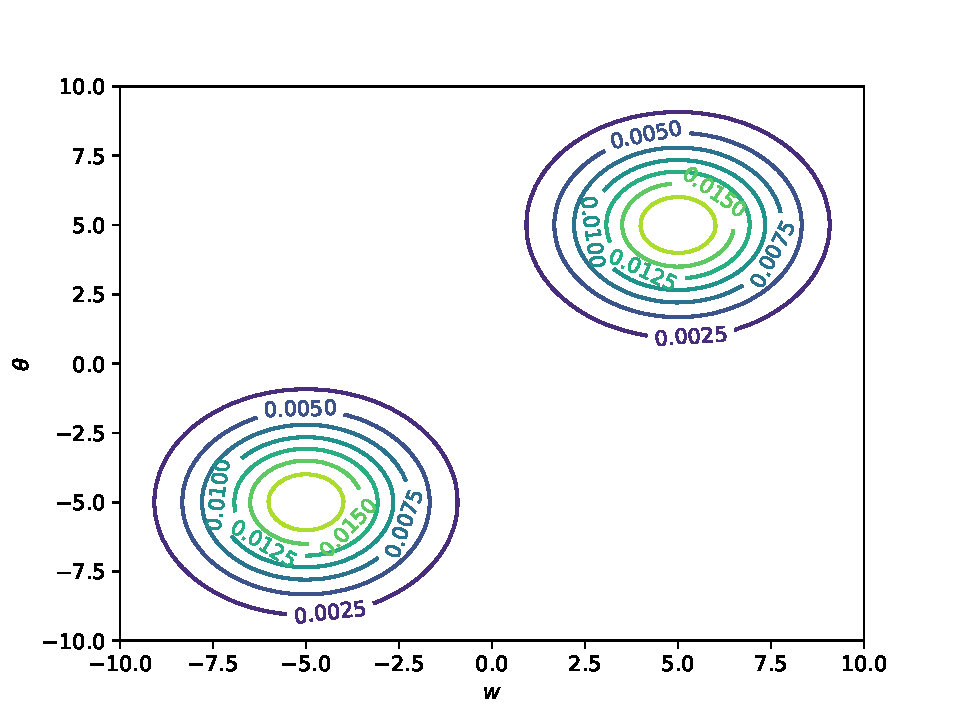
\includegraphics[width=.5\textwidth]{include/figures/plot1}
    \caption{Binormal plot for two strong upward winds}
    \label{fig:plot1}
\end{figure}

However, this bimodal distribution (\autoref{fig:plot1}) doesn't accurately reflect reality.
In nature, we would not expect such a sharp jump between the strong upward winds at $w_1$ and $w_2$.
There would likely be some weaker upward winds present in between.
The current binormal model can attempt to capture this smoother transition by simply increasing the standard deviations of both wind and liquid water potential temperature distributions.
This results in a broader distribution with a connection between the two peaks, as shown in \autoref{fig:plot2}, where $\sigma_w = 5$, $\sigma_{\theta_l1} = 5$, $\sigma_{\theta_l1} = 5$.

\begin{figure}
    \centering
    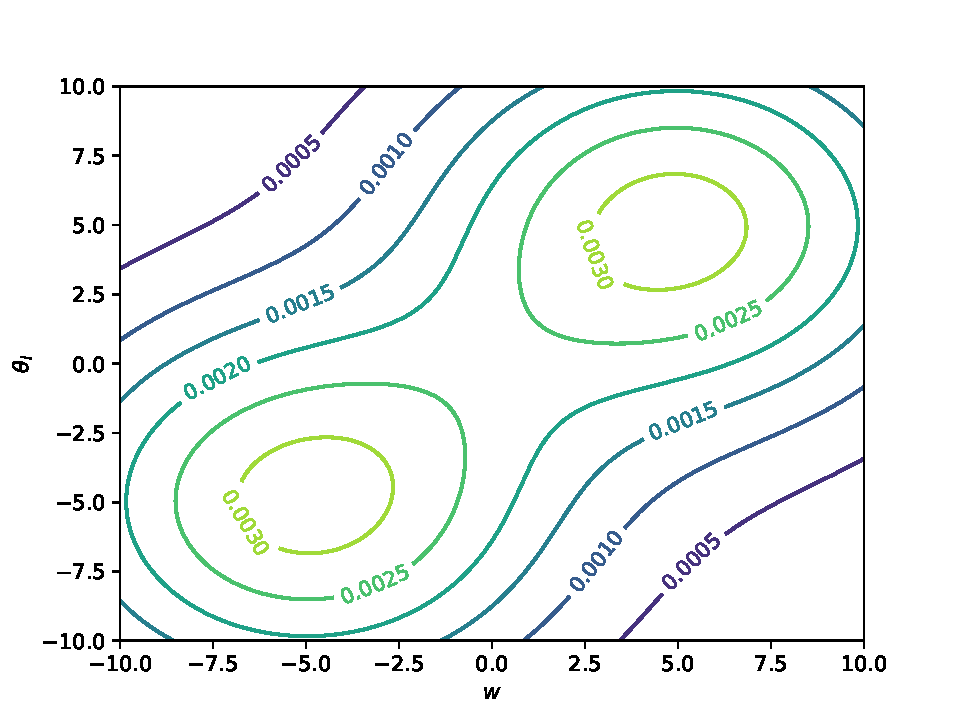
\includegraphics[width=.5\textwidth]{include/figures/plot2}
    \caption{Binormal plot for two strong upward winds with increased standard deviations}
    \label{fig:plot2}
\end{figure}

Seeing this plot, the issue with having some values in the middle is slightly fixed but the general width of the Normals was increased, too.
Since \gls{CLUBB} also has the simplification that there is no correlation between $w$ and $\theta_l$, and $w$ and $r_t$, obviously one cannot just increase this.
Therefore, the idea is to add this third Normal, which actually has correlation between all three variables and especially in the bivariate case, between $w$ and $\theta_l$.
The previous plot would then change to \autoref{fig:plot3}, where $\sigma_w = 2$, $\sigma_{\theta_l1} = 2$,  $\sigma_{\theta_l1} = 2$, $\sigma_{\lambda_w} = 2$, $\sigma_{\lambda\theta_l} = 2$.

\begin{figure}
    \centering
    \begin{tabular}{cc}
        \multicolumn{1}{c}{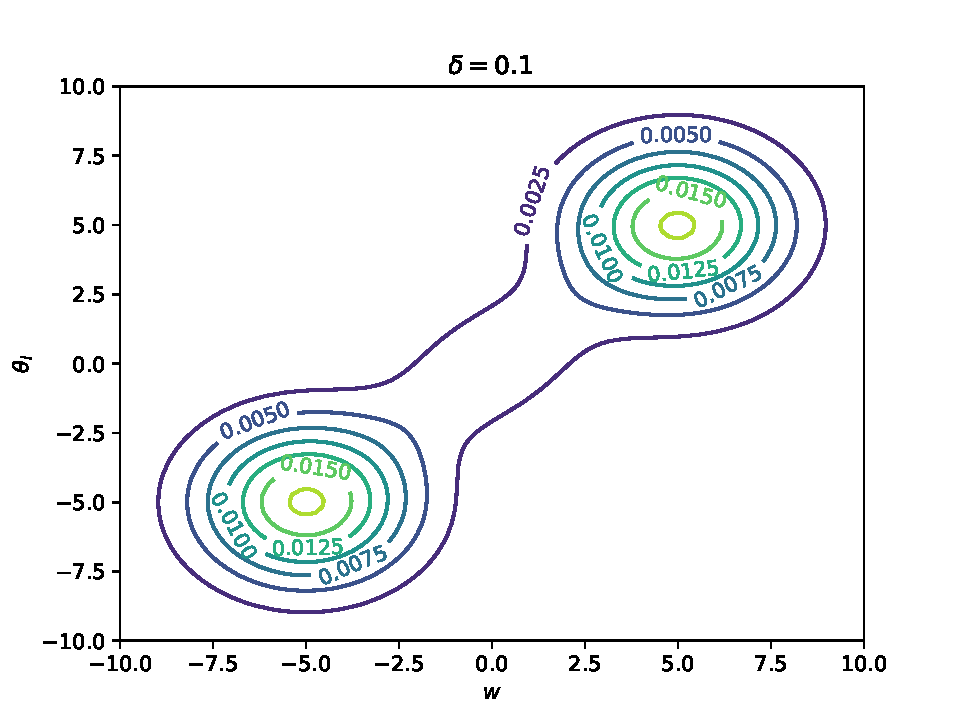
\includegraphics[width=0.48\textwidth]{include/figures/plot3_1}} &
        \multicolumn{1}{c}{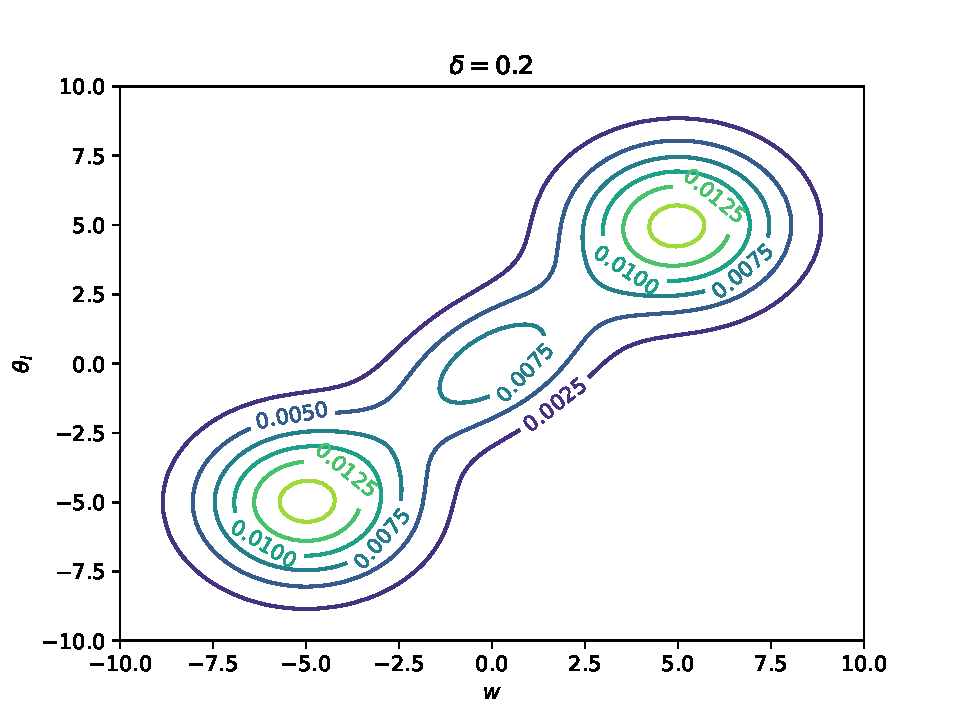
\includegraphics[width=0.48\textwidth]{include/figures/plot3_2}} \\
        $\delta = 0.1$ & $\delta = 0.2$ \\ \\
        \multicolumn{1}{c}{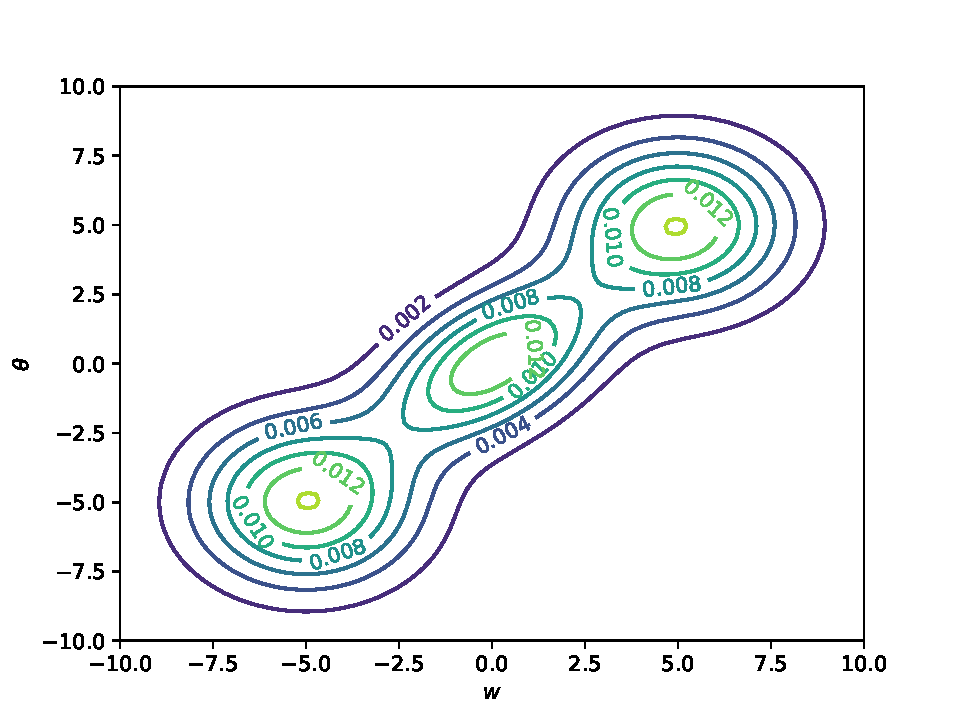
\includegraphics[width=0.48\textwidth]{include/figures/plot3_3}} &
        \multicolumn{1}{c}{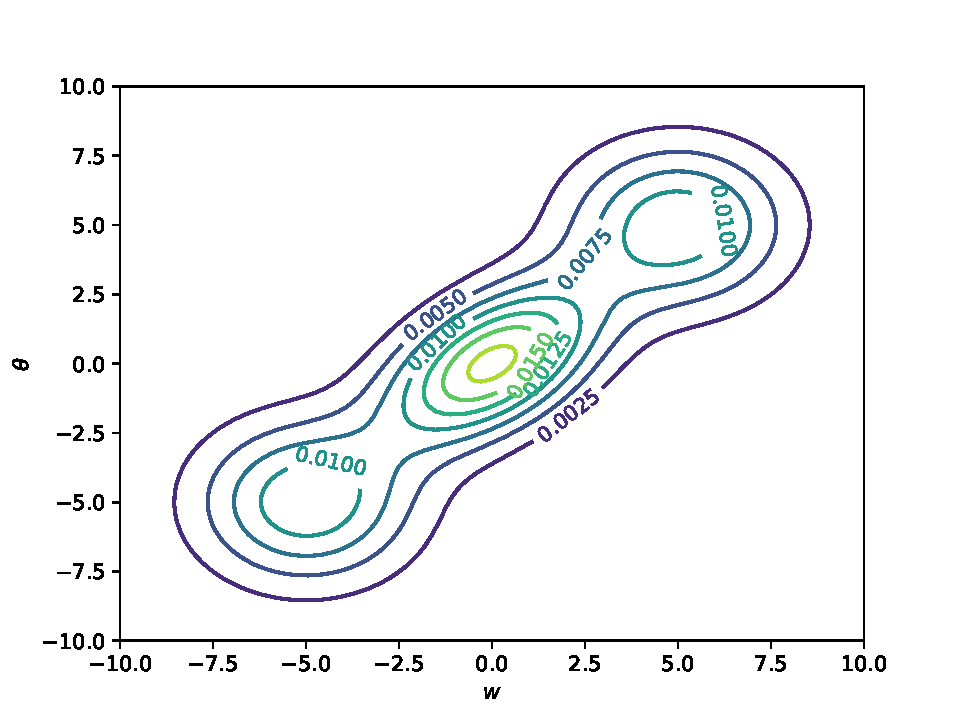
\includegraphics[width=0.48\textwidth]{include/figures/plot3_4}} \\
        $\delta = 0.3$ & $\delta = 0.4$
    \end{tabular}
    \caption{Trinormal plot for two strong upward winds with varying $\delta$}
    \label{fig:plot3}
\end{figure}

Now, one can easily model something like the described shape.
Also, some other (maybe weird) shapes are now possible, just like the following in \autoref{fig:plot4}.

\begin{figure}
    \centering
    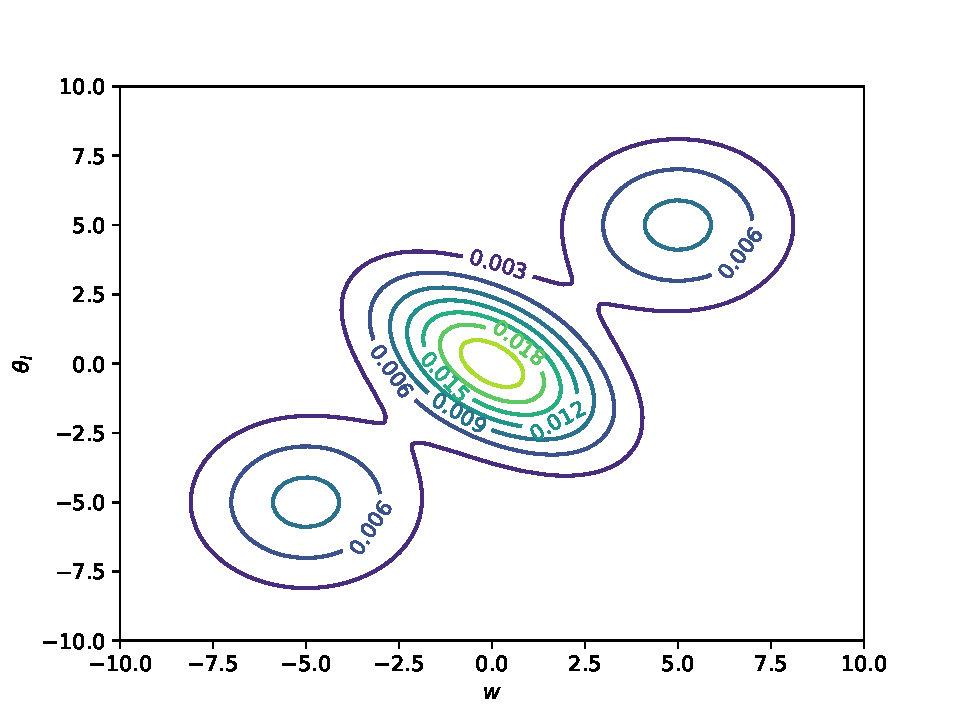
\includegraphics[width=.5\textwidth]{include/figures/plot4}
    \caption{Trinormal plot for two strong upward winds with a third peak in the middle}
    \label{fig:plot4}
\end{figure}